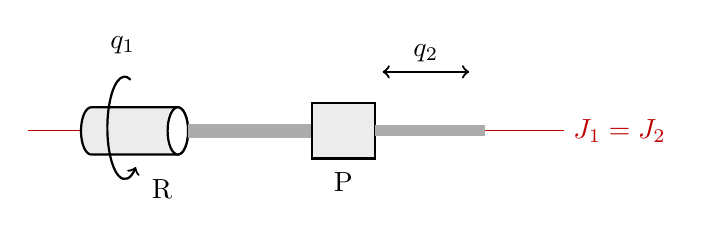
\begin{tikzpicture}
\draw[red!75!black] (-.8,0)--(6,0) node[right] {$J_1=J_2$};
\path[draw,thick,fill=gray!15] (0,-.3)--(1.1,-.3)
 arc[start angle=-90,end angle=90,x radius=.13,y radius=.3]
 --(0,.3) arc[start angle=90,end angle=270,x radius=.13,y radius=.3];
\draw[fill=white,thick] (1.1,0) ellipse (.13 and .3);
\draw[line width=5pt,gray!65] (1.23,0)--(2.8,0);
\draw[fill=gray!15,thick] (2.8,-.35) rectangle (3.6,.35);
\draw[line width=4pt,gray!65] (3.6,0)--(5,0);
\draw[<->,thick] (3.7,.75)--(4.8,.75) node[midway,above] {$q_2$};
\draw[->,thick] (.5,.65) arc[start angle=70,end angle=310,x radius=.22,y radius=.65];
\node[above] at (.4,.85) {$q_1$};
\node[below] at (.9,-.5) {R};
\node[below] at (3.2,-.4) {P};
\end{tikzpicture}
